\section{Seconde formulation robuste}
\subsection{Modèle}
Le modèle robuste linéaire se base sur le pire des cas possible pour calculer un $epsilon$ optimal. On impose maintenant que
$$\sum_{i=1}^N \xi_i^2 \leq \gamma^2$$
On veut choisir une valeur de $\gamma$ telle que $P(\sum_{i=1}^N \xi_i^2 \leq \gamma^2)\geq 0.9999$. On va utiliser ici des variables intermédiaires $\xi_i^2$. La moyenne et la variance de ces variables sont $\mu = \frac{\tau^2}{3}$ et $\sigma^2 = \tau^4\cdot(\frac{1}{5}-\frac{1}{9})$.
Par le théorême central limite, on sait que la distribution $Z = \sum_{i=1}^N \xi_i^2$ tend vers une variable normale : $Z\sim \mathcal{N}(N\mu, N\sigma^2)$. Il suffi alors d'inverser la CDF de Z pour trouver $\gamma$ tel que $P(Z\leq \gamma^2)=0.9999$( v. table \ref{gamma} pour les résultats).
\begin{table}
\centering
\begin{tabular}{|c|c|c|}
\hline
$\tau$ & 0.001 & 0.01 \\
\hline
$\gamma$ & 0.0045107 & 0.045107 \\
\hline
\end{tabular}
\caption{Résultat de nos calculs pour $\gamma$}
\label{gamma}
\end{table}
%TODO : vérifier
On s'attend donc à de meilleurs résultats car les zones de $\mathbb{R}_N$ où tous les $\xi_i$ ont une valeur absolue élevée sont supprimées.
On peut à nouveau reprendre les contraintes du primal et reformuler un problème d'optimisation, conique cette fois. On écrit à nouveau une paire primal dual :
\begin{center}
\begin{minipage}{0.4\textwidth}
\begin{eqnarray}
\max_{\xi} dx^T \xi & \leq & \epsilon - d(\theta)^Tx \nonumber \\
\begin{pmatrix}t \\ \xi \end{pmatrix} & \in  & \mathbb{L}_{R^{n+1}} \nonumber \\ 
t = \gamma \nonumber
\end{eqnarray}
\end{minipage}
\begin{minipage}{0.4\textwidth}
\begin{eqnarray*}
\min_{y} \gamma^2 y & \leq & \epsilon - d(\theta)^Tx \\
\begin{pmatrix}
y \\
d_1(\theta)x_1(\theta) \\
\vdots \\
d_n(\theta)x_n(\theta)
\end{pmatrix}
 & \in & \mathbb{L}_{R^{n+1}}
\end{eqnarray*}
\end{minipage}
\end{center}
Par la dualité forte, l'objectif optimal du dual conique est supérieur à l'optimum du primal. Celà nous permet encore une fois de réécrire notre problème de façon conique :
\begin{center}
\begin{minipage}{0.4\textwidth}
\begin{eqnarray*}
\min_{x,\epsilon ,y_1,y_2,y_3,y_4} \epsilon & & \\
y_{i}(\theta) & \geq & 0 \\
\begin{pmatrix}
y_i(\theta) \\
d_1(\theta)x_1(\theta)\\
\vdots \\
d_n(\theta)x_n(\theta)
\end{pmatrix}
& \succeq_{\mathbb{L}^{N+1}}& 0\\
\forall i = 1,2,3,4 &
\forall \theta \in S_e \cup P_e & \\
\end{eqnarray*}
\end{minipage}
\vline
\begin{minipage}{0.4\textwidth}
\begin{eqnarray*}
\gamma^2 y_{1}(\theta) & \leq & \epsilon -d(\theta)^Tx \\
\gamma^2 y_{2}(\theta) & \leq & \epsilon + d(\theta)^Tx \\
\forall \theta \in S_e & & \\
\gamma^2 y_{3}(\theta) & \leq & \epsilon +1 -d(\theta)^Tx \\
\gamma^2 y_{4}(\theta) & \leq & \epsilon -1 + d(\theta)^Tx \\
\forall \theta \in P_e & &
\end{eqnarray*}
\end{minipage}
\end{center}

\subsection{Analyse des résultats}
La figure \ref{fig:D-ModCon} montre nos résultats pour différents types de perturbation. On constate que notre modèle résiste aux perturbations mais qu'un nombre non-négligeable de réalisations de $\hat{D(\theta)}$ dépasse les bornes imposées. Celà est sans doute du à l'approximation que nous avons faite pour calculer la valeur de $\gamma$.
\begin{figure}[h!]
  \centering
  \begin{subfigure}[b]{0.32\textwidth}
  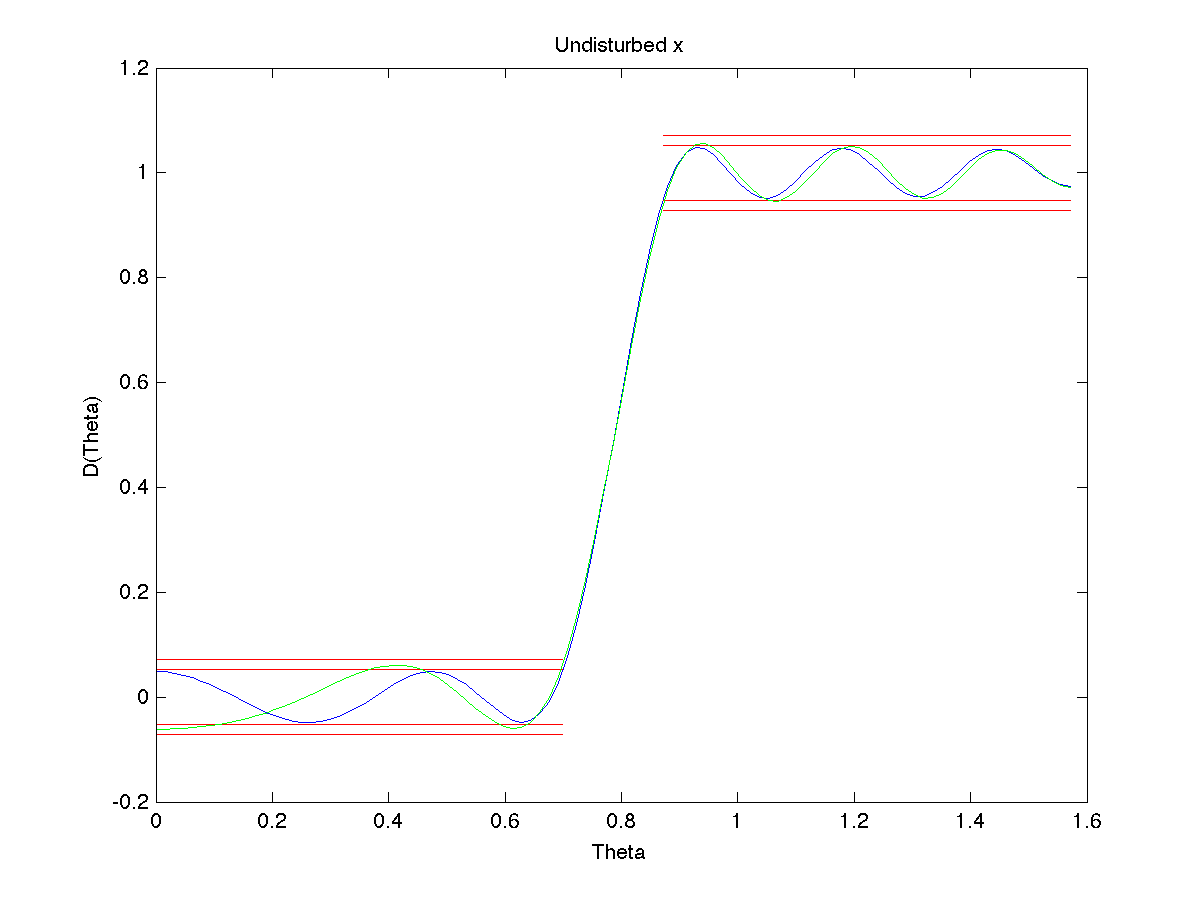
\includegraphics[width=\textwidth]{D-ModRobustCon.png}
  \end{subfigure}
  ~ 
 \begin{subfigure}[b]{0.32\textwidth}
  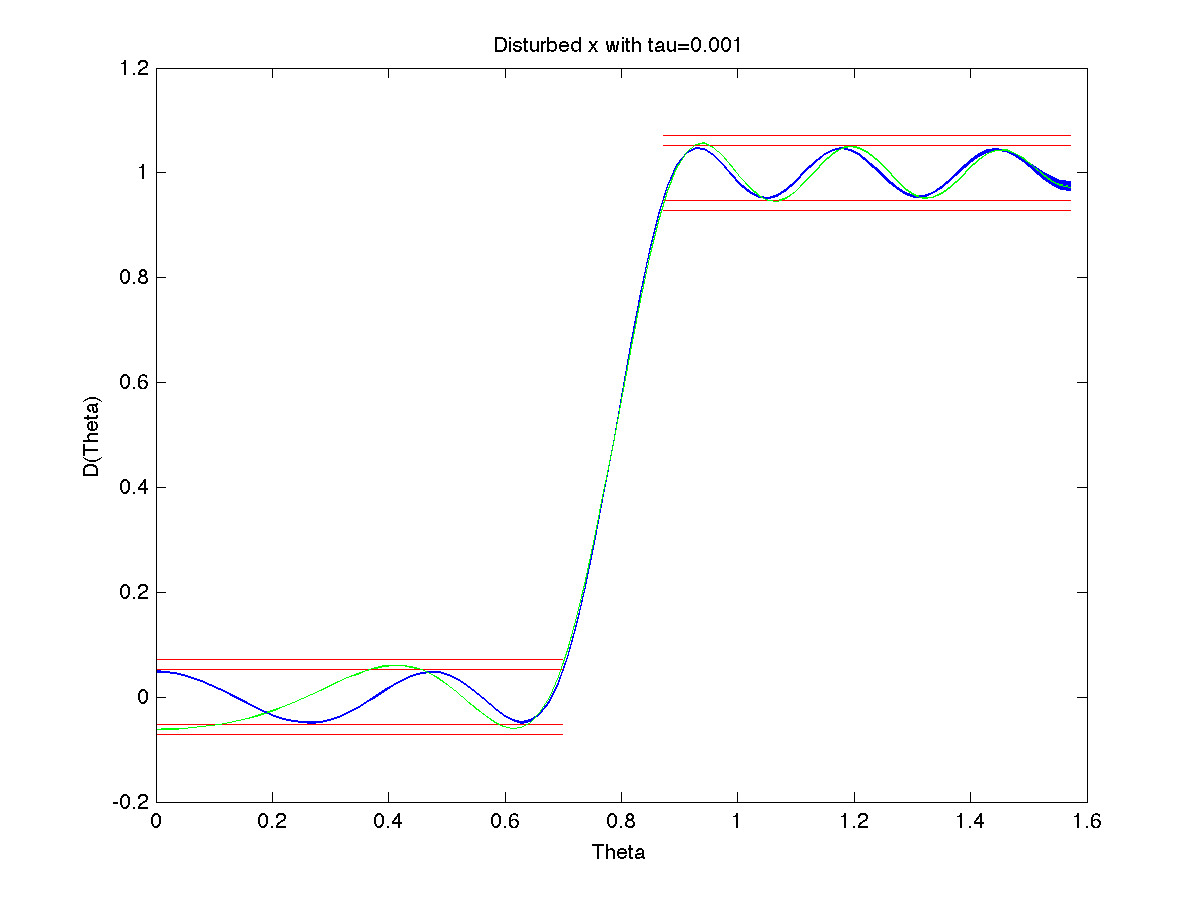
\includegraphics[width=\textwidth]{D-ModRobustCon-tau0001.png}
  \end{subfigure}
  \begin{subfigure}[b]{0.32\textwidth}
  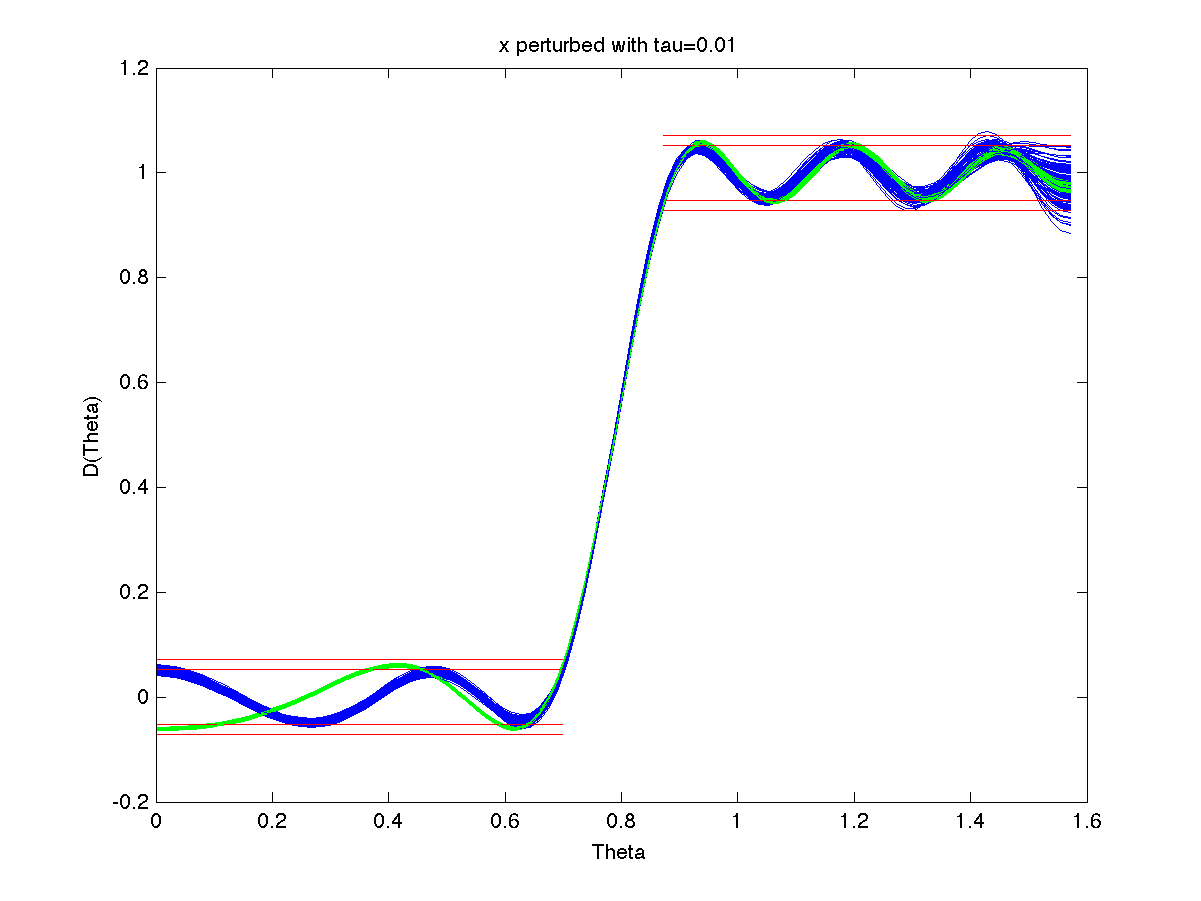
\includegraphics[width=\textwidth]{D-ModRobustCon-tau001.png}
  \end{subfigure}
\caption{Graphes de $D(\theta)$ pour des $x$ non-perturbés, avec une perturbation $\tau=0.001$ et avec une perturbation $\tau = 0.01$(en vert pour un modèle de $\tau=0.01$ en bleu pour $\tau=0.001$). Les deux derniers graphes sont donnés pour une centaine de réalisations des $\xi_i$.}
  \label{fig:D-ModCon}

  \end{figure}
